\documentclass[a4paper,12pt]{article}

\usepackage{natbib,setspace,amsmath,graphicx,float,booktabs}
\usepackage[skip=0.5\baselineskip]{caption}
\usepackage[title]{appendix}

\onehalfspacing
\newcommand{\bs}[1]{\boldsymbol{#1}}
\setlength\parindent{0pt}

\begin{document}

\begin{titlepage}
\noindent
\includegraphics[width=5cm]{uzh_logo_e_pos.pdf}
\noindent{\bf Department of Economics}
\noindent\rule{\textwidth}{0.4pt}
\vspace{1cm}
  \begin{center}
		  {\LARGE Causes of economic fluctuations in the interwar United States. VAR application in the AS-AD framework  \\}
		{\Large Quantitative Economic History - Applications\\Spring Term 2021}
  \end{center}
\vfill

{\flushleft
Hubert Mrugala \\
Banking and Finance\\
hubert.mrugala@uzh.ch\\
19764265}  

\end{titlepage}

\pagebreak
\pagebreak

\section{Introduction}

The interwar period was a very interesting and eventful time of a new monetary and political regime. Economic indicators around the globe were very volatile and the USA was no exception. From 1919 to 1940, the economy of United States have experienced some painful and acute declines in economic activity: Depression of 1920-21, The Great Depression, Recession of 1937-38. The country also underwent 1920s boom and post Great Depression (GD) recovery.

It would be interesting to see what was the main reason for the volatility in prices, especially the collapse in 1930s (see figure \ref{fig:1}). In the AS-AD framework the fall in prices could be explained by either positive supply shock or negative demand shock. Each statement is plausible. For example, one can argue that it was the fall in prices of raw materials in the periphery (emerging markets), thus oversupply, that then forced the prices of goods in developed countries to plummet. Another rationale is that the prices went down because of insufficient aggregate demand. Stop in lending in 1928 \citep{kindleberger1973} or inappropriate monetary policy \citep{friedman1963} could be a cause of decline in demand, and so the falling prices.

To examine whether AD or AS shock was responsible for the volatility in prices in the interwar USA, I use a vector autoregression (VAR) model with two time-series of Industrial Production (IP) and Consumer Price Index (CPI). To make the model fit the traditional AS-AD model, and also to solve the identification problem, I use Blanchard-Quach decomposition that sets restriction on the long run AS line.


\section{Data}

The dataset consists of 252 monthly observations of American IP and CPI from January 1919 to December 1939. The data can be split into two periods, i.e. pre-Great Depression and Great Depression. The first one I define as the time between the beginning of the data sample, January 1919, to the upper-turning point in May 1929, the second one follows from that point to the end of the time-series. On figure \ref{fig:1} and figure \ref{fig:2} the two periods are separated by a red vertical line. Some simple statistics are shown in the table \ref{table:1}, and a table with yearly data for the time-series can be found in the appendix. 

\begin{table}[h]
\caption{Basic Statistics}
\label{table:1}
\centering
\input{../output/tables/stats.txt}
\end{table}

After the war there was a sharp increase in the price level index from 57 in the beginning of 1919 to 70 in mid 1920s. Then, prices had deflated to about 59 (Depression of 1920-21) and stayed around that level until the Great Depression. In February 1931 CPI dropped below 55. Not surprisingly years 1931-33 are considered to be the most severe time of the Great Depression as in this period prices were rapidly declining each month until reaching the lowest point of 43.7 in April 1933.

\begin{figure}[!htb]
    \centering
\caption{Consumer Price Index}
\label{fig:1}
    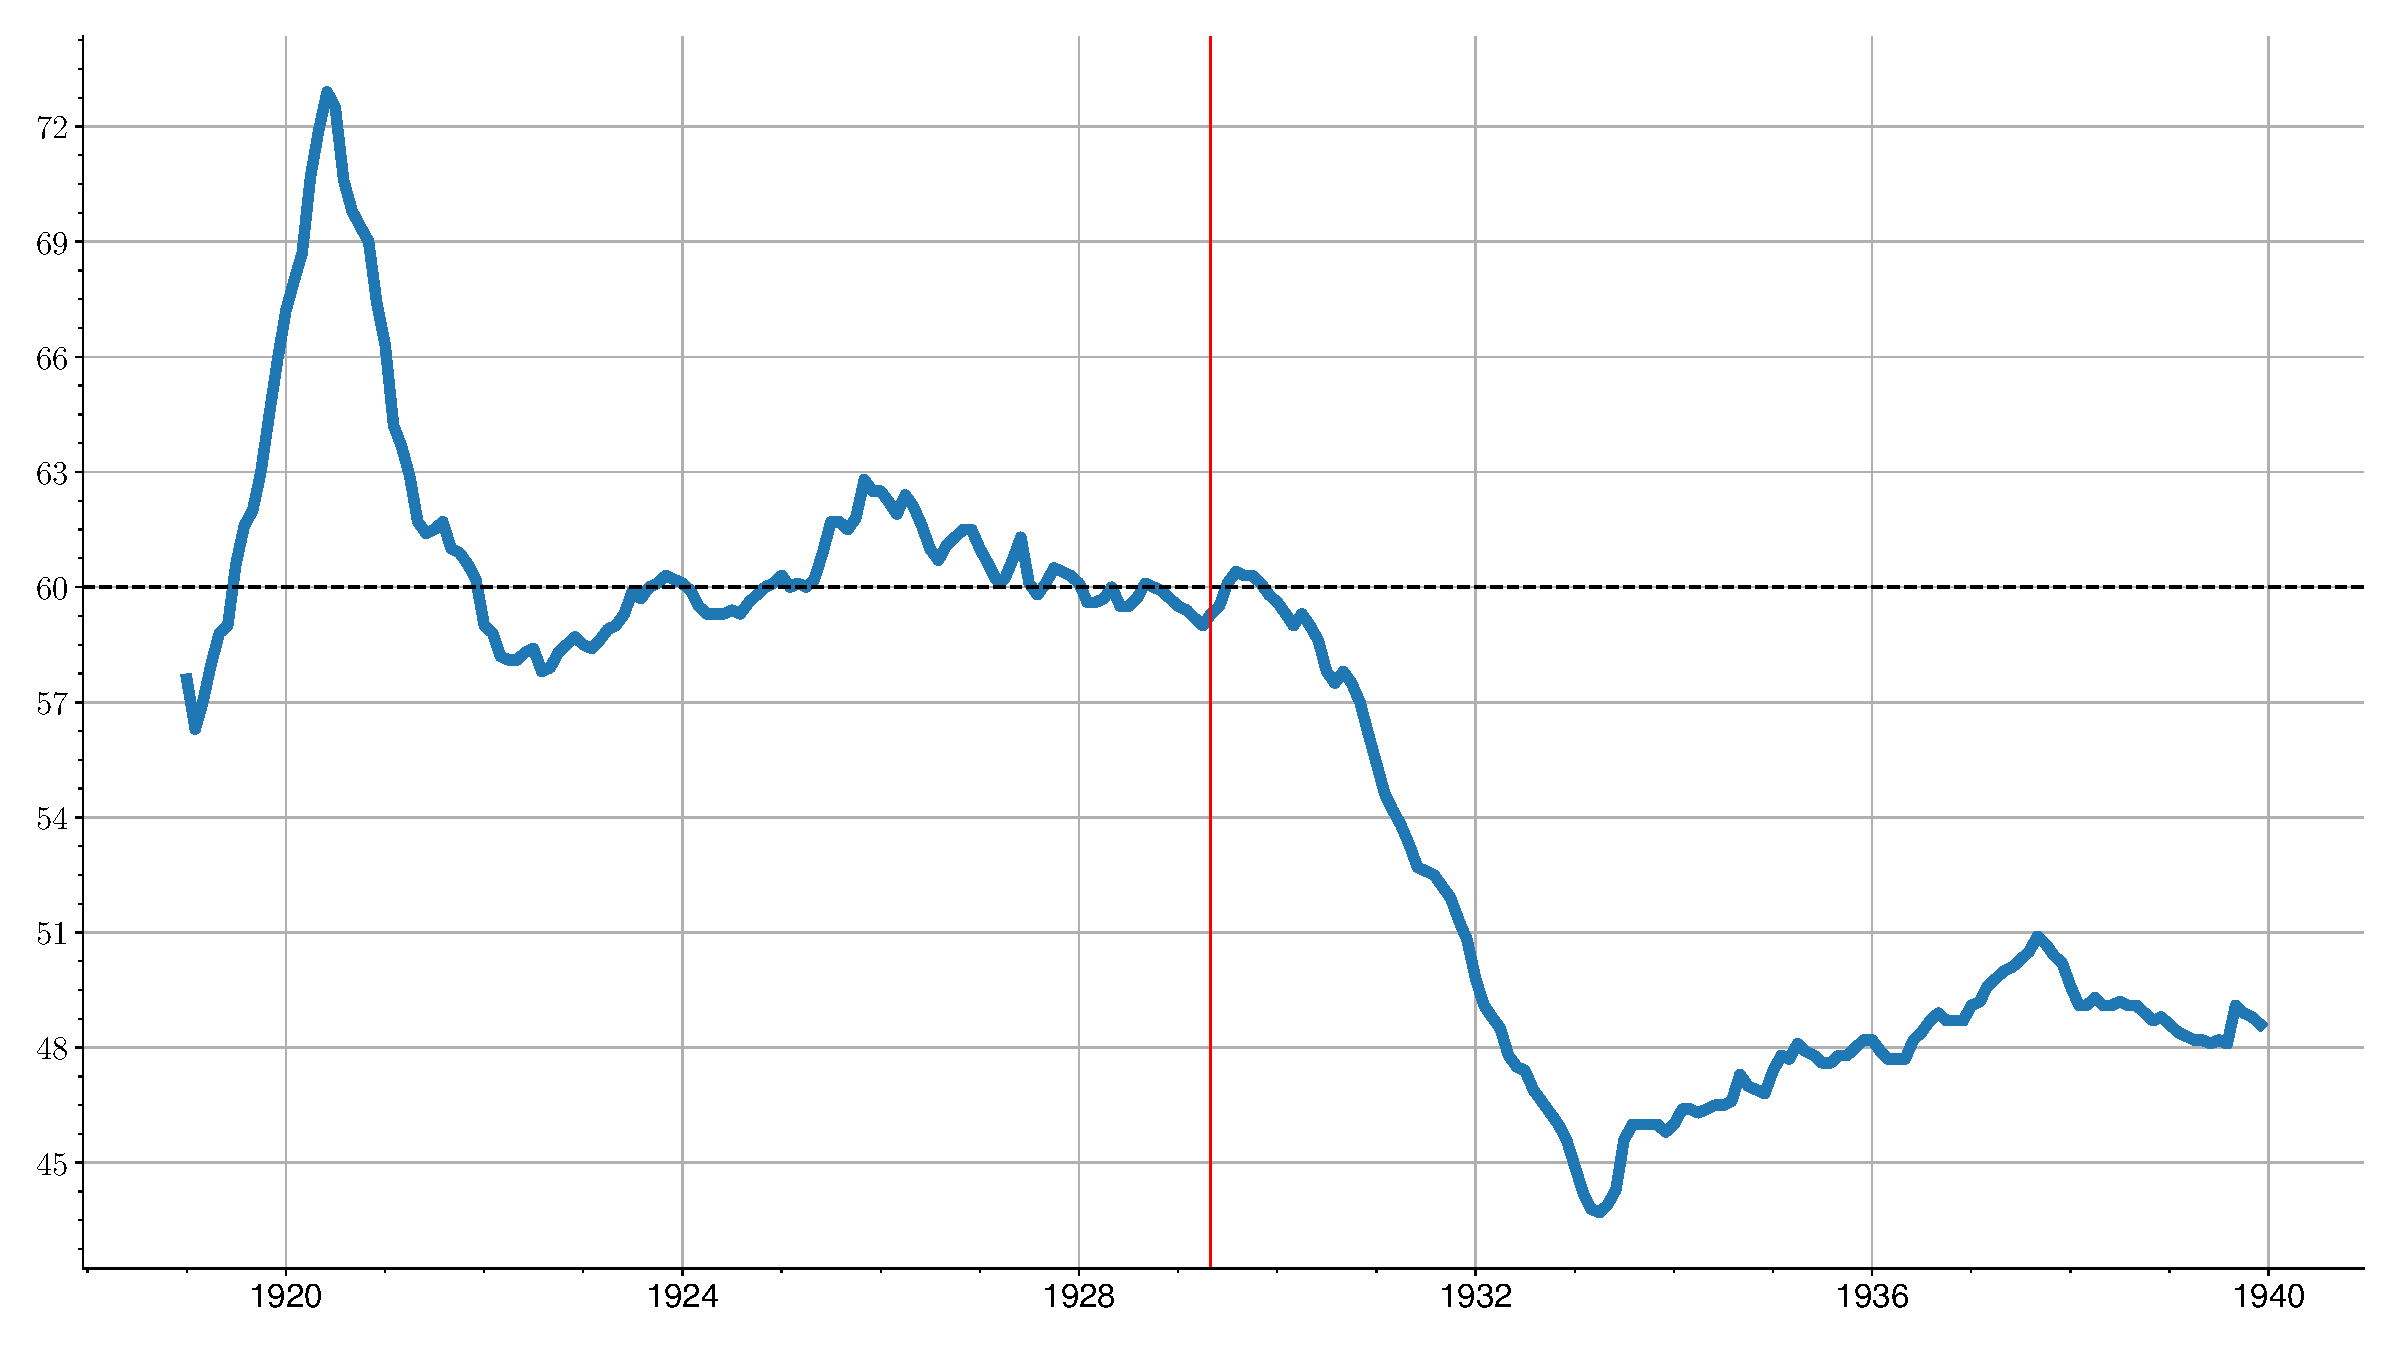
\includegraphics[width=\textwidth]{../output/figures/ts_CPI.pdf} 
\end{figure}

\begin{figure}[!htb]
    \centering
\caption{Industrial Production}
\label{fig:2}
    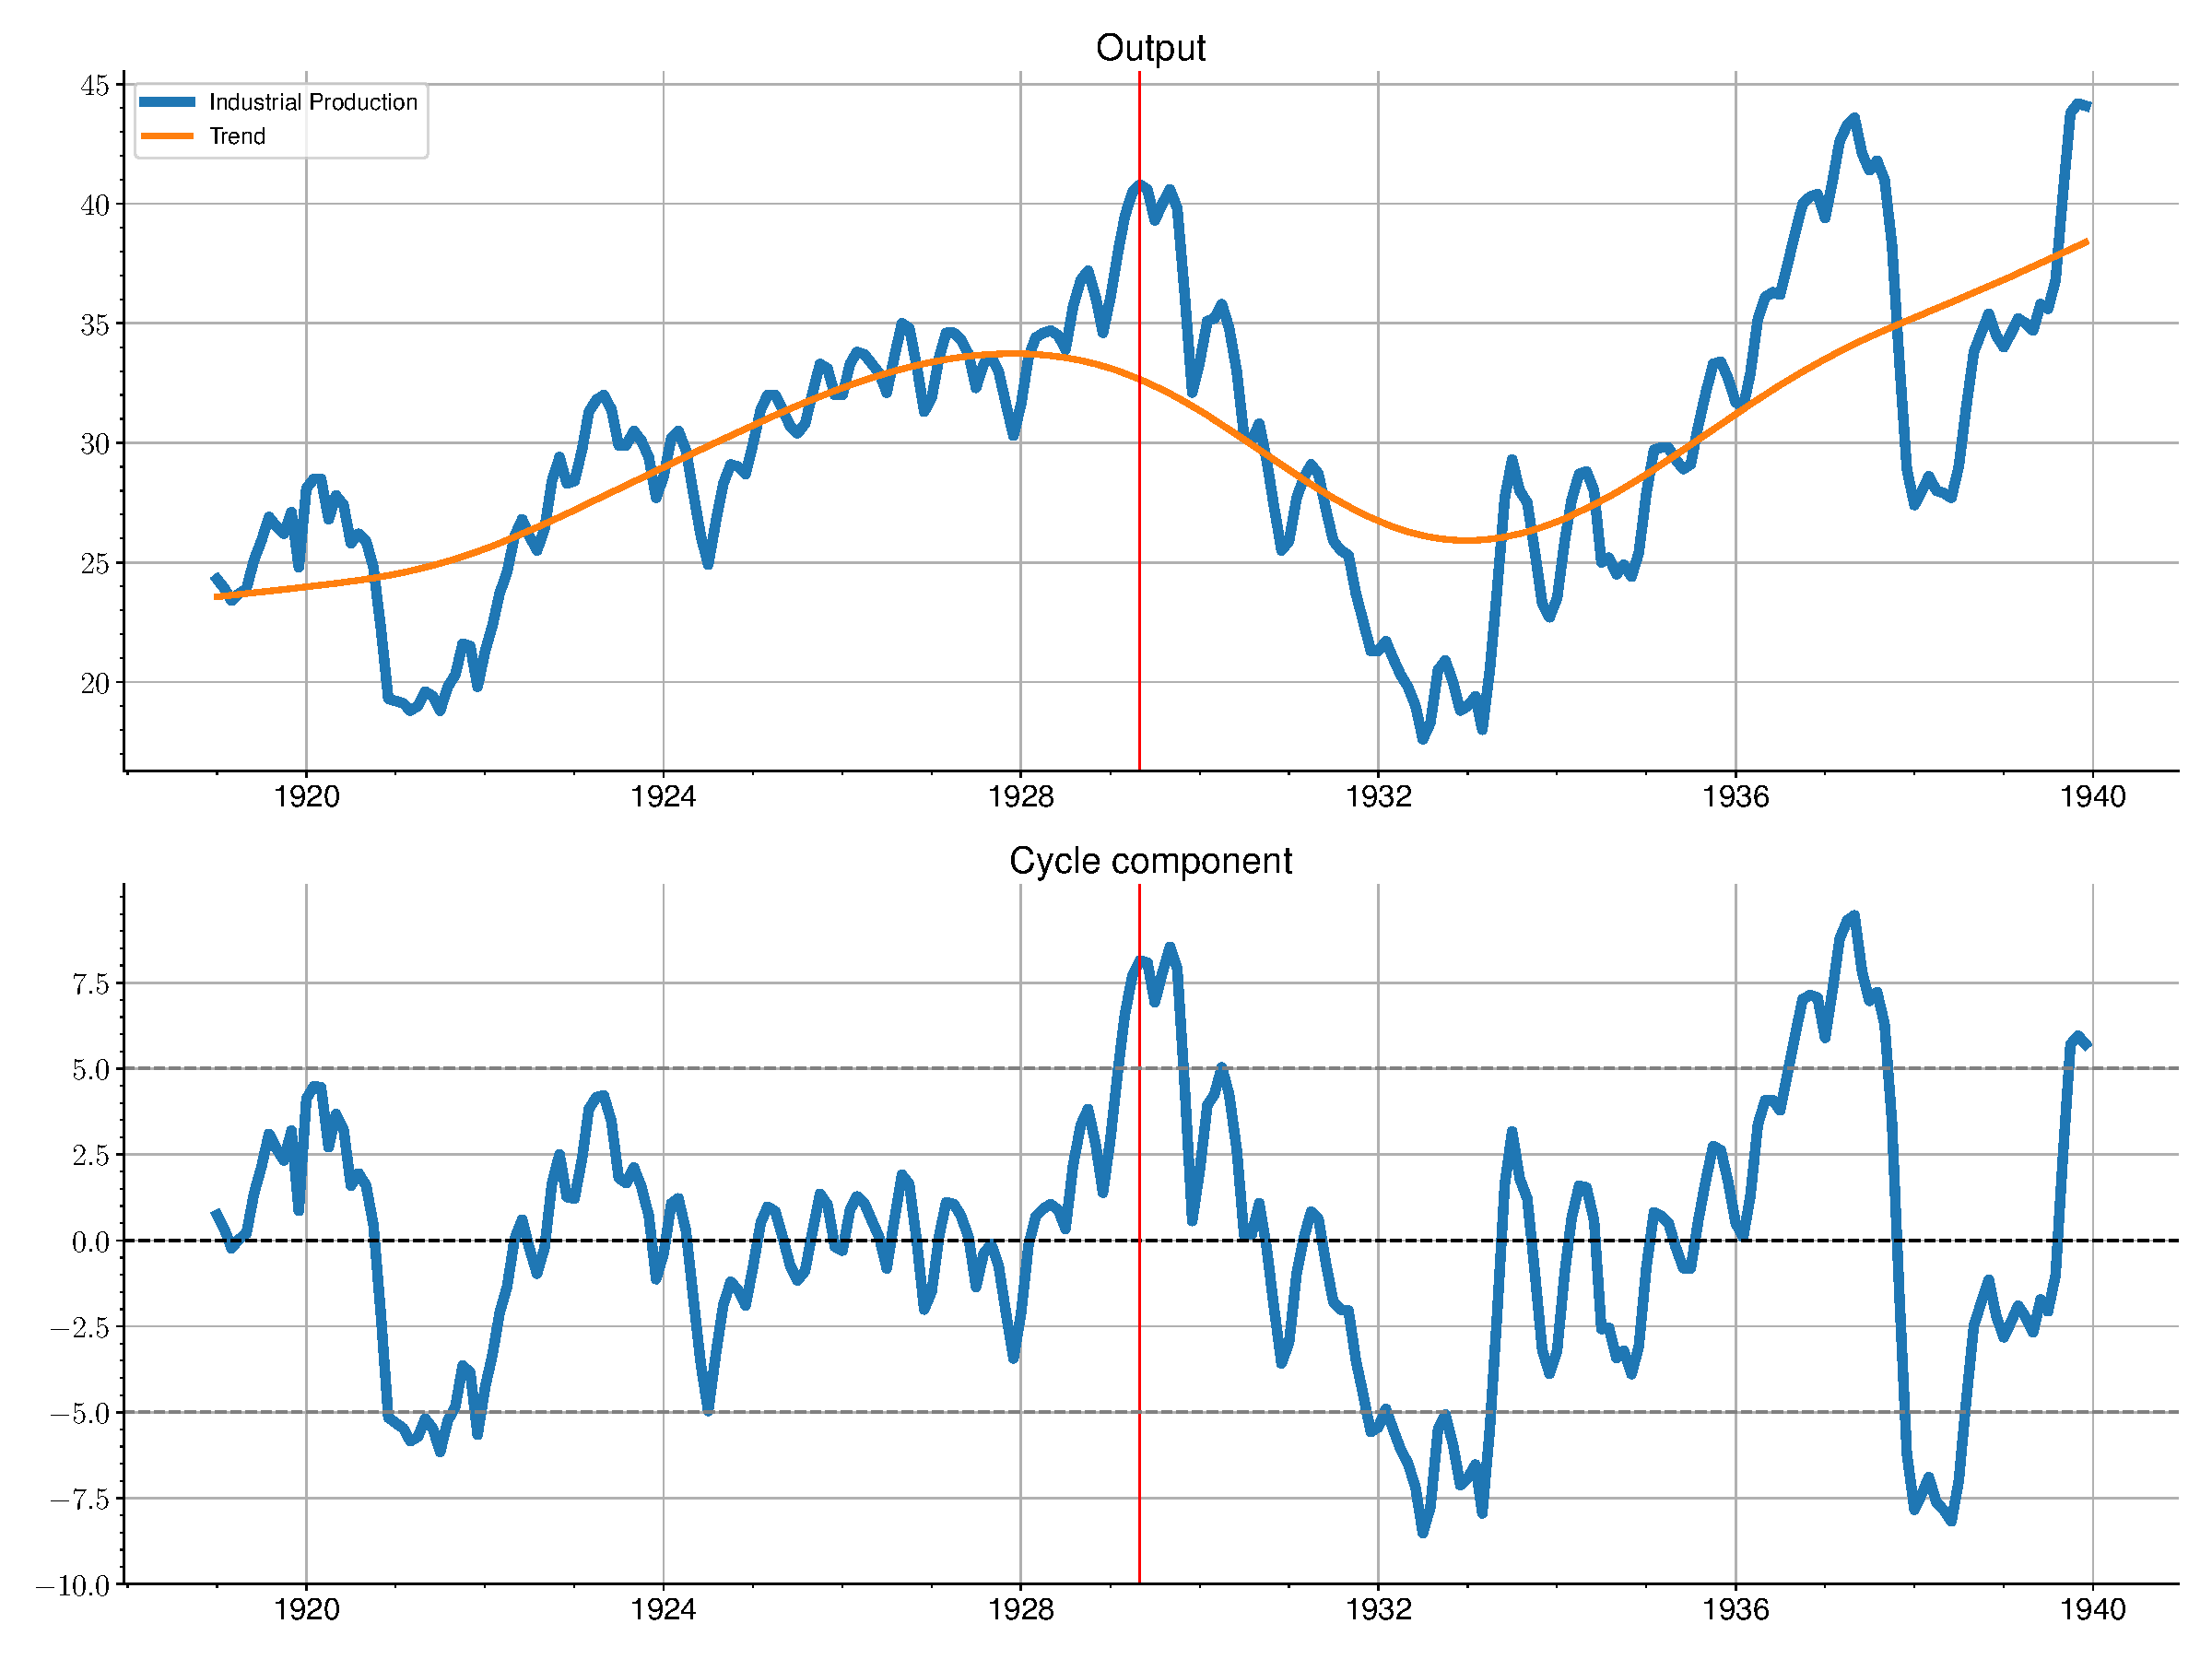
\includegraphics[width=\textwidth]{../output/figures/ts_IP.pdf} 
\end{figure}

Pre-Great Depression Industrial Production, except the time of 1920-21 depression, was growing steadily. At the peak, IP was about 40 and it took almost 7 years of depression and recovery to come back to that level. Recovered production didn't stay that high for long. At the end of the inter-war period we can see a very sudden collapse of IP. It is the Recession of 1937-38. According to \cite{bordo2012} it was the third-worst contraction of the twentieth century. 

To better understand the business cycle in the interwar United States I detrended the time-series with a Hodrick-Prescot filter (see Figure \ref{fig:2}). For the smoothing parameter I went with recommendation of \cite{morten1997} and set \(\mu\) to 129600. There were five periods when Industrial Production deviated by more than 5 points from the trend. However, the most distinct seems to be the interval from 1930 to 1933 when not only the cycle component but also the trend component was falling for a prolonged period of time. 

The dataset comes from:
\begin{itemize}
		\item Statistisches Handbuch der Weltwirtschaft (1936), bearb. im statistischen Reichsamt
Verlag für Sozialpolitik, Wirtschaft und Statistik GmbH, Berlin.
\end{itemize}
 

\section{Method}
\subsection{Vector Autoregressive Model}

To analyze relationship between two endogenous time-series, price level \(\bf M\) and output \(\bf Y\), a vector autoregressive model is used

\begin{equation} \label{eq:1}
		{\mathbf{y_{t}=c+A_{1}y_{{t-1}}+A_{2}y_{{t-2}}+\cdots +A_{p}y_{{t-p}}+e_{t}}}.
\end{equation}

In the formula above \(\bf c\) is a constant, \(\bf A_i\) are coefficient matrices and \(\bf u_i\) are error terms. When analyzing monetary transmission mechanism, VAR can be also expressed in the following form \citep{favero2001}

\begin{equation} \label{eq:2}
\begin{split}
		\mathbf{G}\left(\begin{array}{c}
		\mathbf{Y}_{t} \\
		\mathbf{M}_{t}
		\end{array}\right)=\mathbf{K}(L)\left(\begin{array}{c}
		\mathbf{Y}_{t-1} \\
		\mathbf{M}_{t-1}
		\end{array}\right)+\mathbf{F}\left(\begin{array}{c}
		\epsilon_{\mathbf{Y}, \mathbf{t}} \\
		\epsilon_{\mathbf{M}, \mathrm{t}}
		\end{array}\right).
\end{split}
\end{equation}

In the structural model above matrix \(\bf G\) represents contemporaneous relations among the variables and \(\mathbf{K}(L)\) is the matrix of finite-order lag polynomial. The model is not directly observable, however, a reduced form can be estimated

\begin{equation} \label{eq:3}
\begin{split}
		\left(\begin{array}{c}
		\mathbf{Y}_{t} \\
		\mathbf{M}_{t}
		\end{array}\right)=\mathbf{G}^{-1} \mathbf{K}(L)\left(\begin{array}{c}
		\mathbf{Y}_{t-1} \\
		\mathbf{M}_{t-1}
		\end{array}\right)+\mathbf{G}^{-1} \mathbf{F}\left(\begin{array}{c}
		\epsilon_{\mathbf{Y}, \mathbf{t}} \\
		\epsilon_{\mathbf{M}, \mathrm{t}}
		\end{array}\right).
\end{split}
\end{equation}

In this paper, vector autoregression is used to obtain impulse responses and forecast error decomposition in the AS-AD framework. To do this, I use Blanchard-Quach decomposition where we assume that aggregate demand shocks has no long run effect on real output \citep{blanchardquah89}. The assumption helps to solve the identification problem by imposing restrictions on the impact matrix \(\bf S = G^{-1}-F\).


\subsection{Impulse Responses}

Impact matrix \(\bf S\) connects structural shocks \(\bf e_t\) to the reduced form residuals \(\bf u_t\).

\begin{equation} \label{eq:5}
		\mathbf{u}_{\mathbf{t}}=\mathbf{S} \epsilon_{\mathbf{t}}
\end{equation}

To find \(\mathbf{S}\) first lets start with the moving average representations of reduced form VAR (equation 1) and the structural model (equation 2).

\begin{equation} \label{eq:6}
\begin{split}
		\mathbf{y}_{\mathbf{t}} &=\mathbf{B}(\mathbf{L}) \mathbf{u}_{\mathbf{t}}, \\
		\mathbf{y}_{\mathbf{t}} &=\mathbf{C}(\mathbf{L}) \epsilon_{\mathbf{t}}
\end{split}
\end{equation}

After substituting for \(u_t\) and simplifying

\begin{equation} \label{eq:7}
		\mathbf{B}(L) \mathbf{S}=\mathbf{C}(L).
\end{equation}

The long-run coefficient matrix is \(\mathbf{C}(1) = \mathbf{B}(1)\mathbf{S}\), and so to get \(\bf S\), long run \(\mathbf{C}(1)\) is needed. Postmultiplying \(\mathbf{C}(1)\) with its transpose gives

\begin{equation} \label{eq:8}
		\mathbf{B}(1) \mathbf{S S}^{\prime} \mathbf{B}(1)^{\prime}=\mathbf{C}(1) \mathbf{S}^{-1} \mathbf{S} \mathbf{S}^{\prime}\left(\mathbf{S}^{\prime}\right)^{-1} \mathbf{C}(1)^{\prime}=\mathbf{C}(1) \mathbf{C}(1)^{\prime}.
\end{equation}

Cholesky decomposition of the expression above produces the restricted long-run coefficient matrix \(\mathbf{C}(1)\), that allows to calculate matrix \(\bf S\).

\subsection{Forecast Error Variance Decomposition}

Forecast error variances can be expressed as

\begin{equation} \label{eq:9}
		\mathrm{E}\left[\left(y_{k, t+1}-\hat{y}_{k, t+1}\right)^{2}\right]=\mathbf{e}_{k} \mathbf{\Sigma} \mathbf{e}_{k}^{\prime}=\mathbf{e}_{k} \mathbf{S S}^{\prime} \mathbf{e}_{k}^{\prime}=\mathbf{e}_{k} \mathbf{C}_{0} \mathbf{C}_{0}^{\prime} \mathbf{e}_{k}^{\prime}.
\end{equation}

Then contribution of the shock \(l\) to the forecast error variances of variable \(k\) at time \(h\) can be, generally, written in a for of the following three dimensional array

\begin{equation} \label{eq:10}
		\theta_{h, k l}=\frac{\sum_{j=0}^{h-1}\left(\mathbf{e}_{k} \mathbf{C}_{j} \mathbf{e}_{l}^{\prime}\right)^{2}}{\sum_{j=0}^{h-1} \mathbf{e}_{k} \mathbf{C}_{j} \mathbf{C}_{j}^{\prime} \mathbf{e}_{k}^{\prime}}
\end{equation}

\subsection{Model parameters}

The order that is applied to the VAR model is \(p = 12\). Constant is included. Forecast horizon for impulse responses is \(h=30\)

\section{Results}

The long run equilibrium response matrix \(\mathbf{C}(1)\) shows that the output, in the long run, reacted only to the supply shock. The reason for that outcome is the AS-AD assumption implemented by using Blanchard-Quach decomposition. On the other hand, prices reacted positively to both supply and demand shock.

\begin{table}[h]
\label{table:2}
		\caption{Restricted Long Run Responses (in \%)}
\centering
\input{../output/tables/C1.txt}
\end{table}

Figure \ref{fig:3} gives information on the behavior of impulse response functions in the short run. Demand shocks initially produce an increase in output, just as in the AS-AD framework, and then impulses fall to zero. When it comes to the price level, the long-term effects of the demand shocks on CPI can be seen after 3 months. The period when prices are most sensitive to exogenous shifts in demand is between 10 and 20 months.

\begin{figure}[h]
    \centering
\caption{Impulse Responses}
\label{fig:3}
    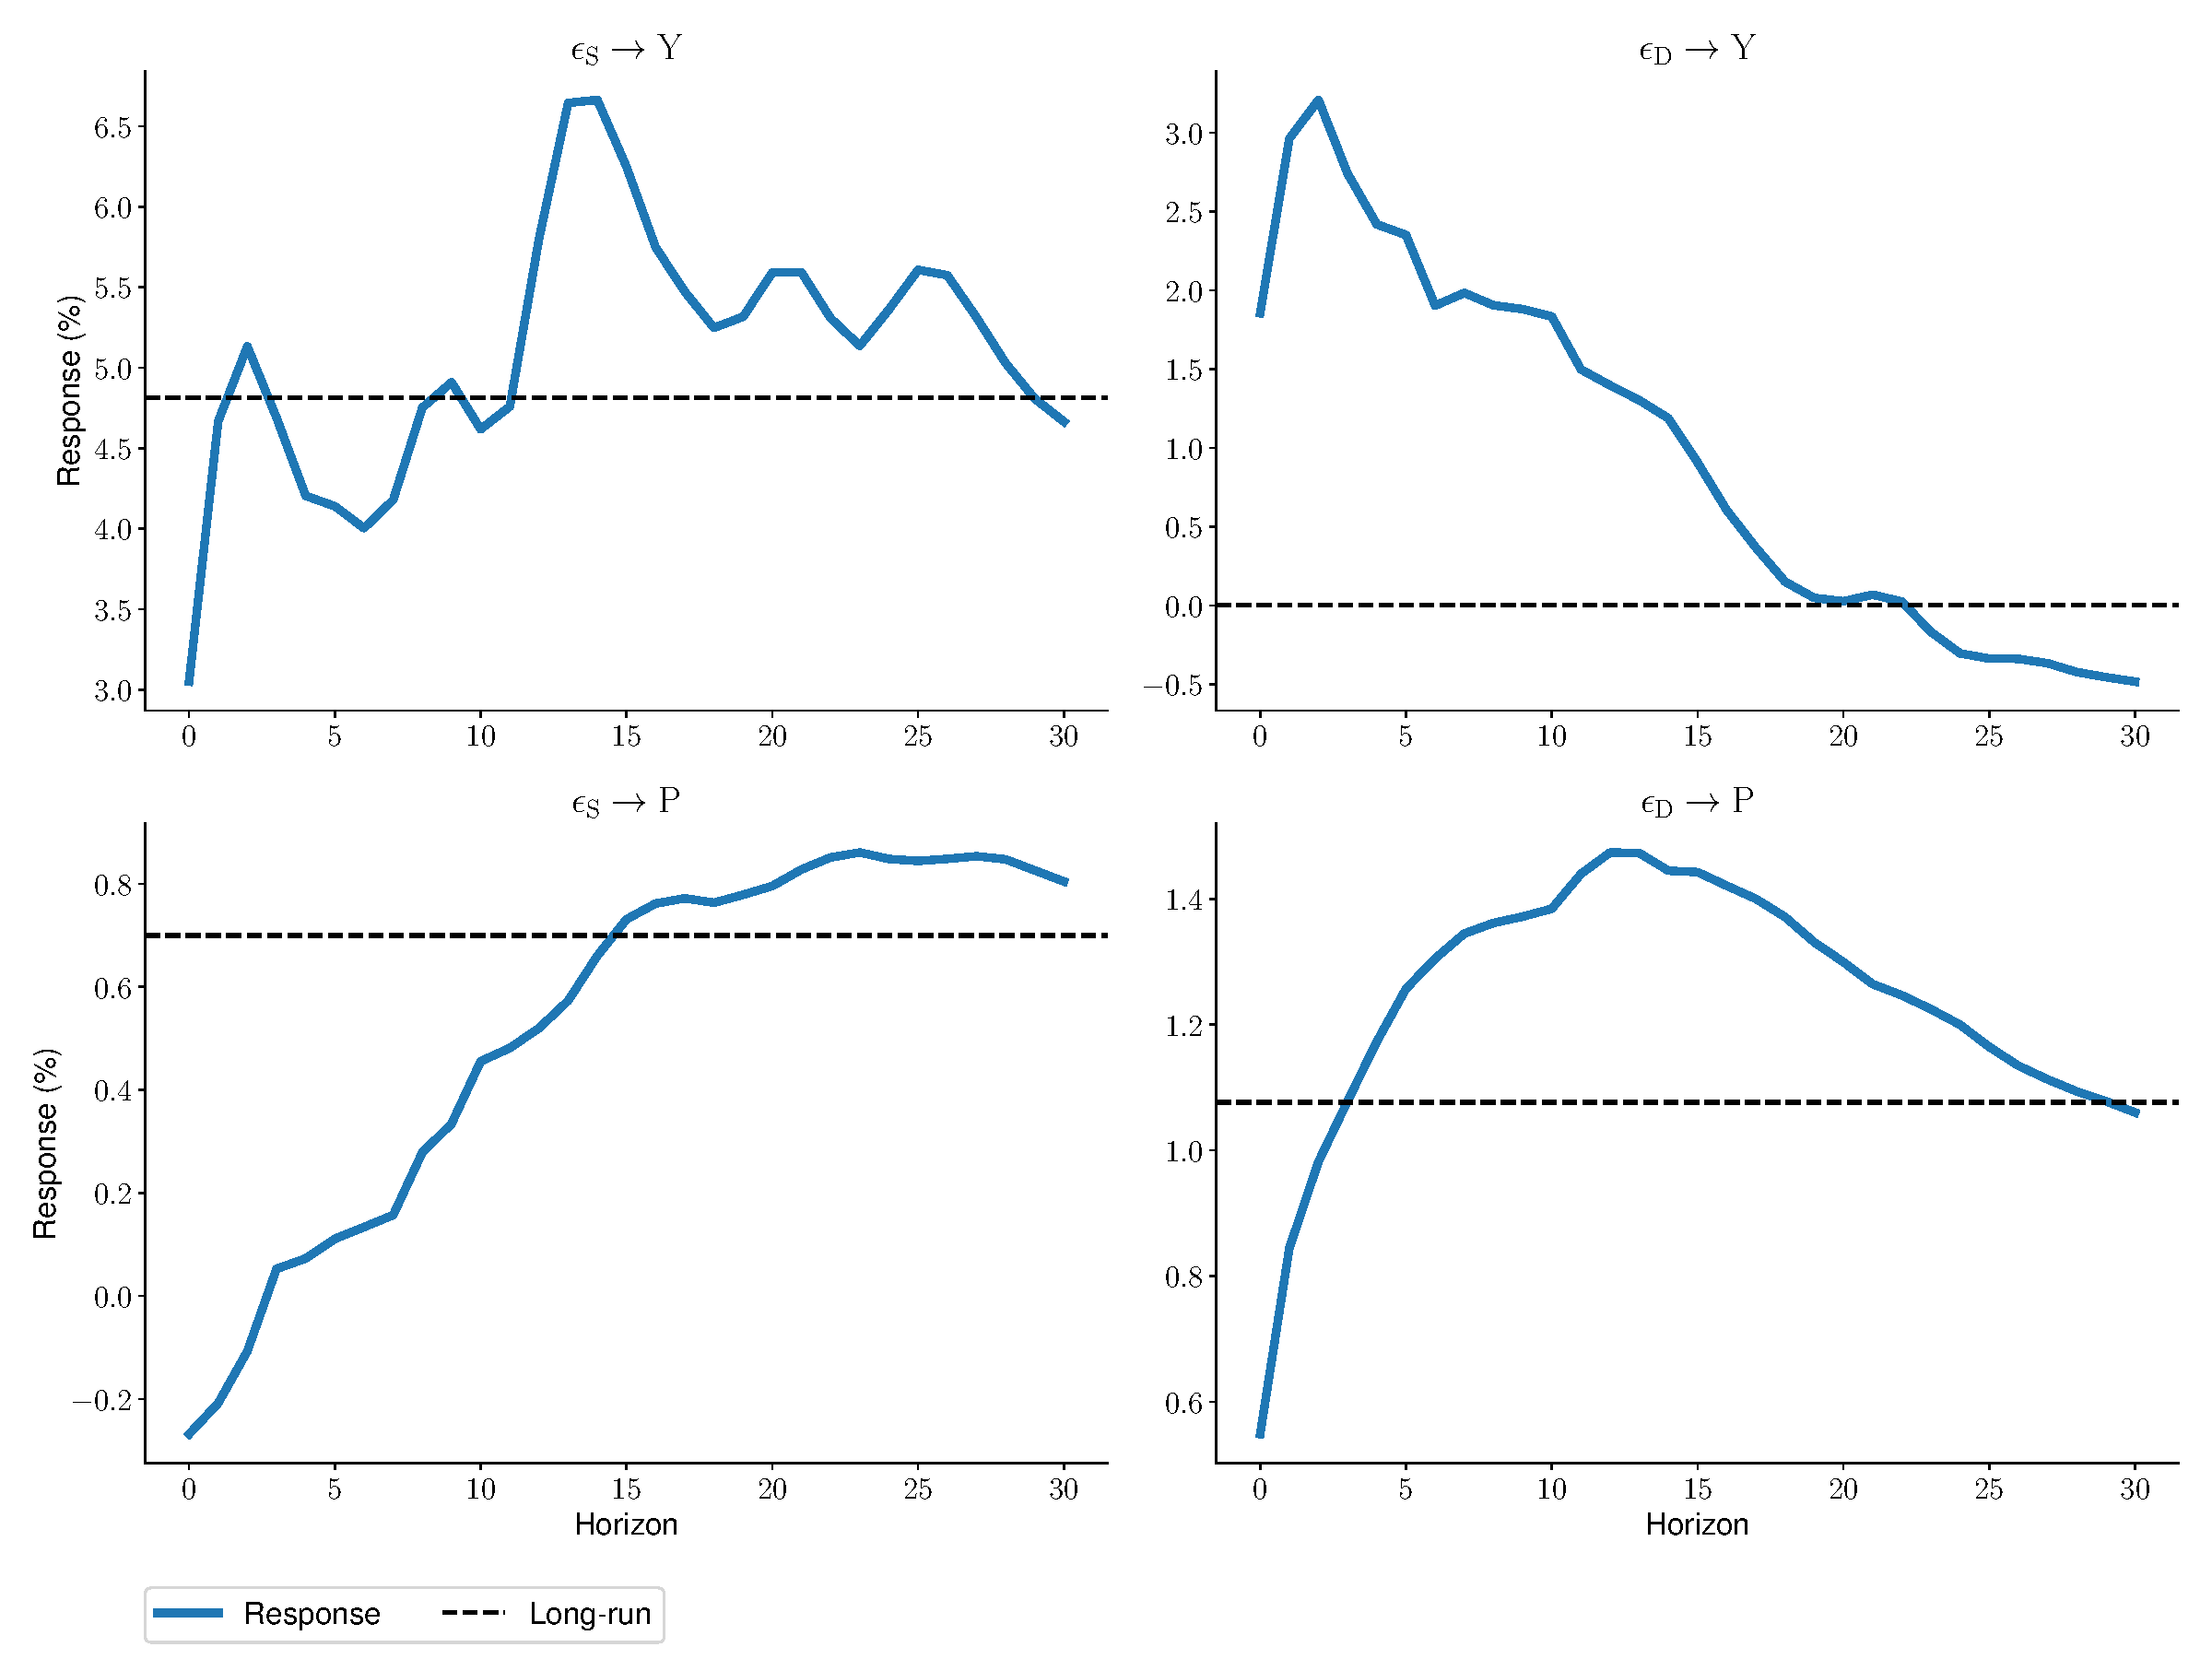
\includegraphics[width=\textwidth]{../output/figures/IR.pdf} 
\end{figure}

\begin{figure}[H]
    \centering
\caption{Forecast Error Variance Decomposition}
\label{fig:4}
    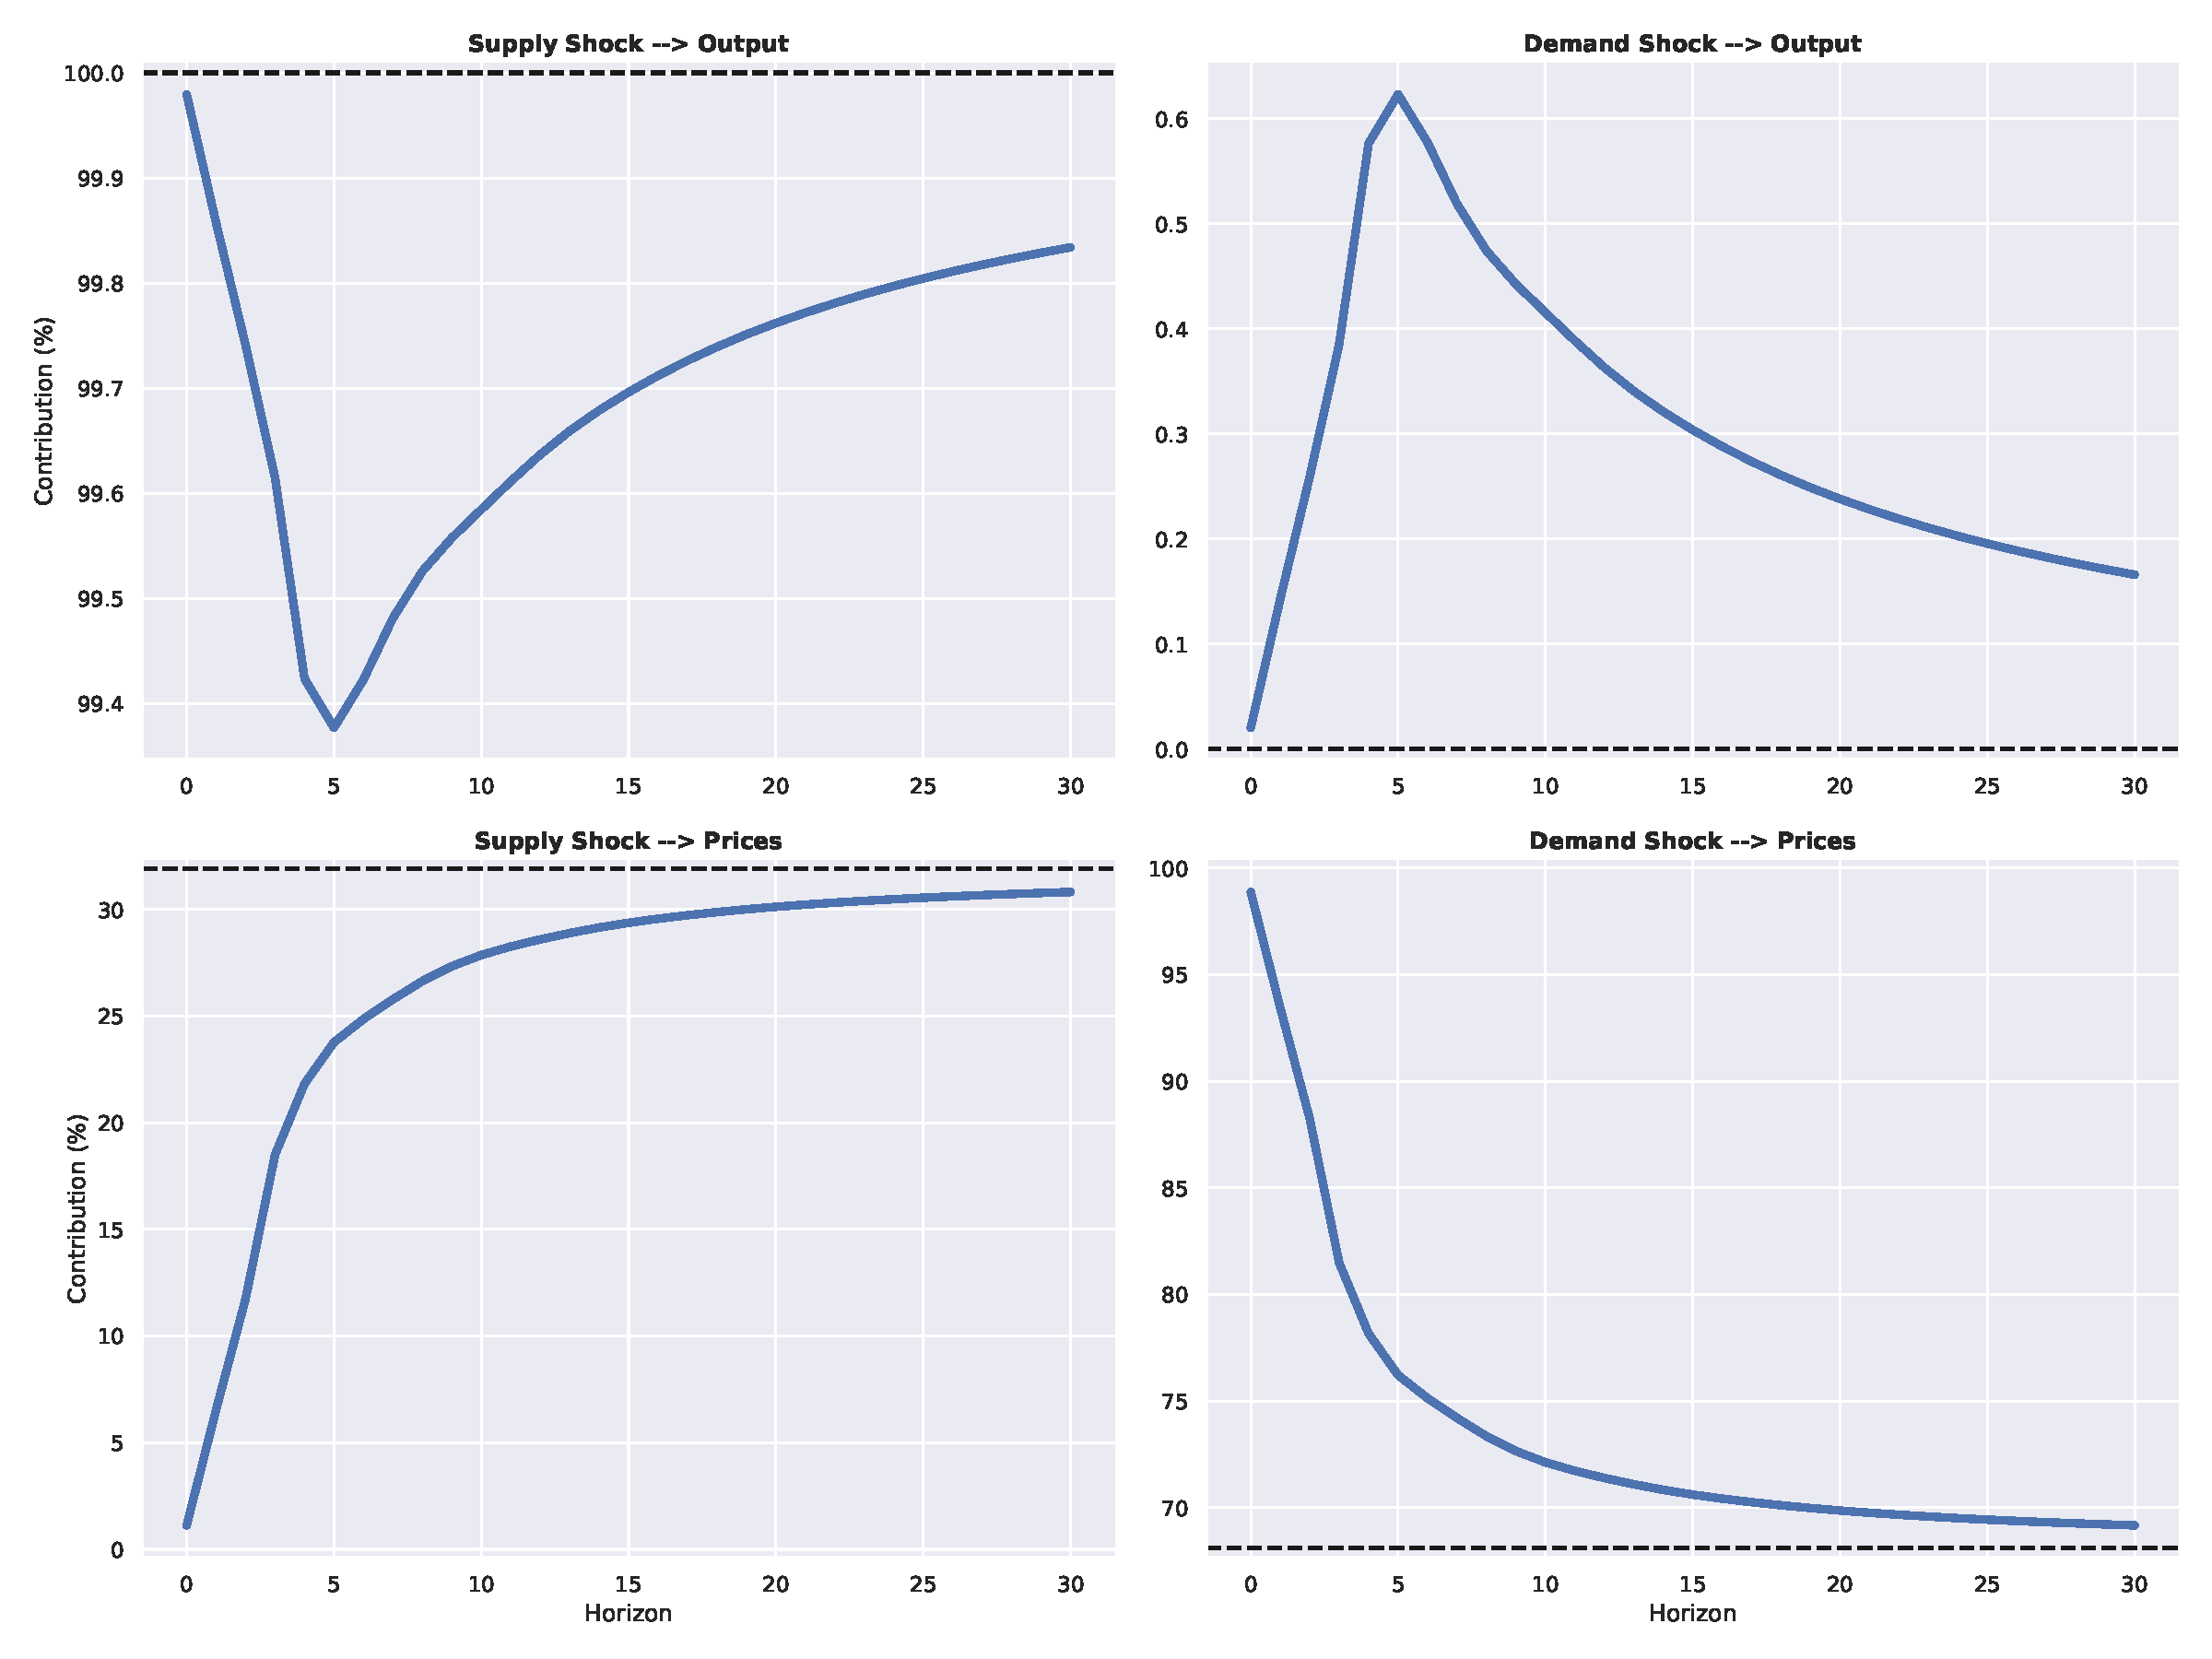
\includegraphics[width=\textwidth]{../output/figures/FEVD.pdf} 
\end{figure}

Figure \ref{fig:4} shows the relative importance of the two shocks over a thirty month horizon (blue lines) and in the long run (dashed lines). FEVD attributes 30\% of changes in prices to supply shocks, and 70\% to demand shocks. For the horizon 0-10, demand shock contribution is much higher than 70\%, and for a long time stays at a level of about 95\%.

The results indicate that high volatility of prices in the interwar USA was caused mainly by demand shocks. These demand shocks could be an effect of inadequate monetary policy, i.e Friedman-Schwarz view, or other monetary effects like halt in lending and gold shortage as described in \cite{kindleberger1973}. Furthermore, it follows that to smooth the business cycle or to make recovery more efficient policy makers should have rather try to adjust aggregate demand, than restraining aggregate supply. 

\pagebreak

\begin{appendices}
\section{Yearly Data}

Data for first January of each year.

\begin{table}[h]
\centering
\input{../output/tables/yearly_data.txt}
\end{table}

\section{Data and the code}

Github repository for the whole project: https://github.com/hmrug/VAR-EconHistory.

\end{appendices}

\pagebreak

\bibliography{sqwg}
\bibliographystyle{eeh}

\end{document}
